\documentclass[conference]{IEEEtran}
\IEEEoverridecommandlockouts
% The preceding line is only needed to identify funding in the first footnote. If that is unneeded, please comment it out.
\usepackage{cite}
\usepackage{amsmath,amssymb,amsfonts}
\usepackage{graphicx}
\usepackage{textcomp}
\usepackage{xcolor}
\usepackage[hidelinks]{hyperref}
\usepackage{float}
\usepackage{booktabs}
\usepackage{array}
\usepackage{pgfplots}
\usepackage{placeins}
\usepackage{tikz}
\usetikzlibrary{positioning,calc,arrows.meta,shapes.geometric,fit,backgrounds}
\pgfplotsset{compat=1.18}
\def\BibTeX{{\rm B\kern-.05em{\sc i\kern-.025em b}\kern-.08em
    T\kern-.1667em\lower.7ex\hbox{E}\kern-.125emX}}
\newcommand{\cmark}{\ding{51}}
\usepackage{pifont}
\usepackage{balance}
\usepackage[ruled,vlined,linesnumbered]{algorithm2e}
\begin{document}


\title{
\fontsize{22}{25}\selectfont
CodeSheriff: Design and Development of an Agentic Security
Auditor for an SFI-Enabled Confidential CI/CD Execution
Layer Using Bayesian Vulnerability Inference
}

\author{\IEEEauthorblockN{Shubhankar Vishnu Patil}
\IEEEauthorblockA{\textit{Dept. of Information Technology} \\
\textit{G H Raisoni College of Engineering and Management}\\
Pune, India \\
shubhankarp258@gmail.com}
\and
\IEEEauthorblockN{Vivek Dnyaneshwar Joshi}
\IEEEauthorblockA{\textit{Dept. of Information Technology} \\
\textit{G H Raisoni College of Engineering and Management}\\
Pune, India \\
vivekdjoshi05@gmail.com}
\and
\IEEEauthorblockN{Yash Suresh Kodgirwar}
\IEEEauthorblockA{\textit{Dept. of Information Technology} \\
\textit{G H Raisoni College of Engineering and Management}\\
Pune, India \\
yashkodgirwar@gmail.com}
\and
\IEEEauthorblockN{Nirmalya Mukhopadhyay}
\IEEEauthorblockA{\textit{Dept. of Information Technology} \\
\textit{G H Raisoni College of Engineering and Management}\\
Pune, India \\
}
\and
\IEEEauthorblockN{Kunal Kundu}
\IEEEauthorblockA{\textit{Dept. of Information Technology} \\
\textit{G H Raisoni College of Engineering and Management}\\
Pune, India \\
}
}

\maketitle

\begin{abstract}
Modern software development increasingly relies
on Continuous Integration/Continuous Deployment (CI/CD) pipelines to deliver software rapidly, but automated
security review at the pull request stage remains limited. Existing
security tools rely on rigid static analysis or homogeneous multi-
agent approaches, which may generate false positives or overlook
complex vulnerabilities. This project will present CodeSheriff, an
agentic security auditor that will analyze GitHub pull requests
using structural, semantic, contextual, and SFI-based confidential
execution analysis. A Bayesian inference engine will fuse evidence
from multiple agents to generate confidence-aware vulnerability
assessments, while an automated patch generation and verifica-
tion module will recommend and validate fixes through GitHub
and a web dashboard. The system will enhance CI/CD security
by delivering reliable, explainable, and statistically grounded
vulnerability detection while reducing manual review effort.
\end{abstract}
\vspace{6pt}
\begin{IEEEkeywords}
vulnerability detection, multi-agent systems, software security,
continuous integration and continuous deployment
\end{IEEEkeywords}


\section{Introduction}
In today’s software industry, developers frequently push code to the main branch through Pull Requests (PRs). However, security analysis of each Pull Request is still largely performed manually, making the review process more time-consuming.Teams either use basic approaches that only catch known, simple mistakes, or they don't have enough time to properly review every pull request. This is a big problem because even one missed vulnerability can put the whole application at risk once the code is merged and deployed. On top of this, attackers are now also targeting the Continuous Integration/Continuous Deployment (CI/CD) that's builds and runs the code.

Solutions that exist today don’t fully solve this problem. Traditional static analysis approaches identify fixed patterns but are unable to catch tricky ones, so they generate a lot of false alarms. Some recent tools use multiple artificial intelligence (AI) agents, but all these agents basically read the same code in the same way, so they don't really give different opinions. when these approaches combine results, they just use simple voting, which doesn't tell you how confident the final answer actually is.

In this paper, we are proposing CodeSheriff to fix this problem. It uses four different types of agents that look at the code from different perspectives. Static agent checks the code structure, the meaning of the code is understood by the semantic agent, the context agent checks whether accepting this PR could bring back any vulnerability from previously accepted PR, and the runtime agent actually watches the code run inside a safe, isolated environment using software fault isolation (SFI). All this information is then combined using a Bayesian model, which gives a clear probability of whether the code is vulnerable, along with how confident the system is. This same safe environment also protects the CI/CD workflow, since it only releases secret keys when it is sure the correct, verified code is running.


The rest of this paper is structured as follows. Section \ref{LS} talks about related work already done in this area. Section \ref{PS} explains our proposed method, its algorithms and its implementation. Section \ref{IMP} describes the experimental evaluation, Section \ref{RES} discusses the results, and Section \ref{CON} concludes the paper.

\section{Literature Survey} \label{LS}

Early learning-based studies explored structural and sequential representations for vulnerability detection. Li and Yang \cite{ref20} compared sequence and graph-based deep learning methods, identifying challenges in capturing long-range dependencies and generalizing to noisy data. CODE-SMASH \cite{ref19} and XTransformer \cite{ref18} employed hierarchical neural and transformer architectures to capture multi-level code representations and improve similarity-based detection, while remaining sensitive to computational cost and dataset characteristics . Abbasi and Shameli-Sendi \cite{ref4} used Code Property Graph metrics with machine learning for interpretable vulnerability and vulnerability-type prediction, but their approach was limited to C/C++. DeepSecure \cite{ref2} combined CodeBERT with bidirectional long short-term memory(BiLSTM) and convolutional neural network(CNN) layers for python vulnerability detection, incorporating robustness and confidence calibration, but remained language-specific and affected by noisy labels.

Transformer and large language model(LLM) based approaches have subsequently improved semantic analysis of source code. Shestov \textit{et al.} \cite{ref13} fine-tuned WizardCoder using parameter-efficient learning for vulnerability classification, but remained limited to function-level analysis. Tamberg and Bahsi and Gnieciak and Szandala \cite{ref14,ref17} benchmarked LLMs against vulnerability detection tasks and traditional static analysis tools, showing strong potential but persistent false positives, hallucinations, localization errors, and inference costs. Gülmez \cite{ref7} surveyed code-generation LLMs and highlighted challenges in structural correctness, repository-level reasoning, and security. Chen \textit{et al.} \cite{ref9} and Su \textit{et al.} \cite{ref8} similarly identified limitations involving context windows, hallucination, dataset quality, generalization, and interpretability. Germano \textit{et al.} \cite{ref10} reviewed LLM-based vulnerability detection, repair, and explanation, noting that research remains more focused on detection than automated repair and explanation.

To address the limitations of isolated code analysis, recent studies have incorporated contextual and repository-level information. Antal \textit{et al.} \cite{ref3} evaluated retrieval augmented generation (RAG) for real-world Java vulnerability detection using retrieved vulnerable and secure examples, but observed false positives and retrieval sparsity. AegisGuard \cite{ref1} incorporated contextual information for semantic vulnerability detection and risk stratification, while SCOUT\cite{ref5} enabled interactive repository exploration to retrieve relevant code context. Göçmen \textit{et al.} \cite{ref15} integrated repository history and dependency analysis into pull-request reviews for change-impact estimation, although static dependency analysis cannot fully capture dynamic behavior.

Multi-agent approaches have further introduced collaborative security reasoning. Wei \textit{et al.} \cite{ref11} used specialized roles and collaborative reasoning for vulnerability auditing, while MAVUL \cite{ref16} combined vulnerability analysis, security architecture review, and iterative evaluation. Reddy \textit{et al.} \cite{ref6} explored knowledge-based agentic AI for automated vulnerability triage, and Syed \textit{et al.} \cite{ref12} investigated an observe--reason--act--verify framework for autonomous software-supply-chain defense. These studies demonstrate the potential of agentic security workflows, while also highlighting challenges such as reduced performance on complex cases, token overhead, and the need for human intervention.

However, existing approaches do not effectively combine structural, semantic and contextual analysis within a unified vulnerability detection framework. We integrate these approaches through specialized agents and confidence-aware vulnerability inference, while providing explanations and patch recommendations within the GitHub pull-request workflow.

% =====================================================================
\section{Proposed Methodology} \label{PS}
% =====================================================================

A vulnerability can hide in the structure of the code, in its intent, in
its departure from the repository's own habits, or only in what the code
does when it runs. To cover these four views, CodeSheriff uses four
independent agents: a Structural agent for data flow, a Semantic agent for
intent, a Context agent for repository precedent, and a Runtime agent for
observed execution. No agent sees the output of another, so their errors
stay independent. A Bayesian inference engine combines their statements
into one \emph{calibrated} probability: a change reported at $87\%$ should
be vulnerable about $87\%$ of the time~\cite{guo2017calibration}.

\subsection{Mathematical Model}

CodeSheriff evaluates a pull request through six stages: change
extraction, structural, semantic, context and runtime analysis, and
Bayesian fusion with the alert decision.

\subsubsection{Change Extraction}
A diff fragment is too small to reason about and a whole file mixes
unrelated code, so the unit of analysis is one changed function. Let
$B_f$ and $H_f$ be the base and head versions of a changed file $f$. The
changed lines and the set of units are
\begin{equation}
L_f=\mathrm{Diff}(B_f,H_f),\qquad
U=\{\,u=\mathrm{Outer}(f,\ell)\;:\;\ell\in L_f\,\}
\label{eq:units}
\end{equation}
where $\mathrm{Outer}(f,\ell)$ is the outermost function of $H_f$ that
contains line $\ell$. Each unit $u$ holds the file, the function name, its
old and new source, and its changed lines. Lines outside any function form
one module-level unit. A unit too large to analyse is never truncated; the
agents abstain on it.

\subsubsection{Structural Agent}
The Structural agent follows data through a definition--use graph from
each function parameter (treated as untrusted) to a dangerous call, or
\emph{sink}, such as \texttt{cursor.execute} or \texttt{os.system}. When an
unsanitised path reaches a sink, the structural score is
\begin{equation}
S_{\mathrm{str}}=\mathrm{clip}_{[0,1]}\bigl(0.45+\delta+0.15\,\nu-0.25\,\rho-0.20\,\theta-\lambda\bigr)
\label{eq:str}
\end{equation}
where $\delta$ is $0.20$ for a critical sink and $0.10$ for a high one,
$\nu=1$ when the code is network-facing, $\rho=1$ when the path passes a
partial sanitizer, $\theta=1$ in a test file, and $\lambda\le0.05$ is a
small penalty for long paths. A second backend, Semgrep~\cite{semgrep},
scores the same unit, and the witness keeps the larger of the two scores,
because both read the same source text.

\subsubsection{Semantic Agent}
Some weaknesses, such as a missing authorization check, have no fixed
syntax. The Semantic agent asks a language model for the intent of the
function, its trust boundaries and the security rule the change breaks.
The model is sampled $n=3$ times, and the score for weakness class $c$ is
the share of samples that report it:
\begin{equation}
S_{\mathrm{sem}}(c)=\frac{m_c}{n}
\label{eq:sem}
\end{equation}
where $m_c$ is the number of accepted samples reporting $c$. A sample is
accepted only when it passes the hallucination gate
\begin{equation}
G(\phi)=[c\in\mathcal{C}]\wedge[\mathrm{file}\ \text{matches}]\wedge[\mathrm{sink}\subseteq\mathrm{src}]\wedge[\mathrm{lines}\subseteq u]
\label{eq:gate}
\end{equation}
where $\mathcal{C}$ is the closed set of ten in-scope CWEs~\cite{cwe}, the
quoted sink must appear word-for-word in the source, and the reported
lines must lie inside the unit. The code is wrapped between random markers
created for each request, so text inside it cannot act as an instruction.

\subsubsection{Context Agent}
A change can be unsafe only because the repository normally does something
else, for example when every similar endpoint checks ownership except the
new one. The Context agent retrieves similar merged functions of the same
repository (384-dimensional local embeddings in pgvector) and reports a
security control $\gamma$ that they apply and the unit does not:
\begin{equation}
\begin{gathered}
S_{\mathrm{ctx}}(\gamma)=b\cdot\min\!\Bigl(1,\frac{\bar{s}}{0.85}\Bigr)\\
b=\begin{cases}0.85,&\text{same function, or } k\ge3\\0.65,&k=2\end{cases}
\end{gathered}
\label{eq:ctx}
\end{equation}
where $\bar{s}$ is the mean similarity of the supporting functions and $k$
is the number of sibling functions that apply $\gamma$. A single sibling
($k=1$) is treated as coincidence and reports nothing. The agent reports
only authorization weaknesses (CWE-862 and CWE-639).

\subsubsection{Runtime Agent}
The Runtime agent executes the changed function once inside a
WebAssembly~\cite{haas2017wasm} sandbox (Wasmtime with WASI), which
provides software fault isolation~\cite{wahbe1993sfi}: there is no network,
no environment and no host file, and fuel, time and memory are capped.
Each parameter $i$ receives a unique random token $t_i$. A value $v$ is
tainted, and a detection is reported, when
\begin{equation}
\mathrm{tainted}(v)\iff\exists\,i:\ t_i\subseteq v,\qquad S_{\mathrm{rt}}=0.85
\label{eq:rt}
\end{equation}
where $v$ is the argument that reaches a sink. A direct observation needs
no graded score, so $S_{\mathrm{rt}}$ is a constant. If the value reached
the sink only because the sandbox had to answer a check it could not
evaluate, the agent abstains instead.

\subsubsection{Bayesian Fusion and Decision}
Every agent $a$ returns one of three statements: a \emph{detection} with a
score $S_a$, a \emph{silence} (it ran and found nothing), or an
\emph{abstention} (it could not run). The statement is placed in a cell
\begin{equation}
z_a=\begin{cases}
\textsc{high}, & S_a\ge0.8\\
\textsc{medium}, & 0.5\le S_a<0.8\\
\textsc{low}, & S_a<0.5\\
\textsc{silence}, & \text{ran, found nothing}
\end{cases}
\label{eq:cell}
\end{equation}
Each cell has a likelihood ratio (LR) fitted on labelled data:
\begin{equation}
\Lambda_a(z)=\frac{P(z\mid V)}{P(z\mid\neg V)}\approx
\frac{(k_V+1)/(N_V+4)}{(k_S+1)/(N_S+4)}
\label{eq:lr}
\end{equation}
where $k_V$ and $k_S$ count vulnerable and safe examples that fell in cell
$z$, and $N_V$ and $N_S$ are the totals. Adding one (Laplace smoothing)
avoids division by zero. An abstention, or a cell never observed, has
$\Lambda=1$, so an agent that could not look never changes the result.
Each LR is clipped to $[0.05,20]$. Starting from the prior $\pi$, the
posterior probability of a vulnerability $V$ given the evidence $E$ is
\begin{equation}
P(V\mid E)=\frac{O}{1+O},\qquad
O=\frac{\pi}{1-\pi}\prod_{a=1}^{4}\Lambda_a(z_a)
\label{eq:post}
\end{equation}
where $O$ is the posterior odds. The product always has four factors, one
per agent, and silences contribute factors below $1$, so the probability
can fall as well as rise. The finding is finally labelled
\begin{equation}
\mathrm{Verdict}=\begin{cases}
\text{Alert},& P(V\mid E)\ge\tau\\
\text{No alert},& \text{otherwise}
\end{cases}
\label{eq:verdict}
\end{equation}
where $\tau=0.227$ is selected on the validation split.

\textit{Worked example.} With $\pi=0.03$ the prior odds are $0.031$. A
medium structural detection ($\Lambda=15.56$), a high semantic detection
($9.48$), a context abstention ($1$) and a high runtime detection ($6.92$)
give $O\approx31.6$ and $P(V\mid E)\approx0.97$. A high semantic detection
alone, with the other three agents abstaining, gives exactly $0.227$: the
threshold means that one strong finding nobody contradicts is just enough
to alert.

\subsection{Algorithms}

The framework is implemented as three algorithmic stages: evidence
generation by the agents, Bayesian fusion, and patch verification.

\begin{algorithm}[t]
\small
\caption{Evidence Generation for One Unit}
\label{alg:agents}
\KwIn{Changed function $u$}
\KwOut{Statements $E=\{e_{\mathrm{str}},e_{\mathrm{sem}},e_{\mathrm{ctx}},e_{\mathrm{rt}}\}$}
\ForEach{agent $a$ in \{Structural, Semantic, Context, Runtime\}}{
  \uIf{$a$ cannot run on $u$ (timeout, no tool, too large)}{
    $e_a\gets$ Abstention(reason)\;
  }
  \Else{
    $F\gets$ findings of $a$ on $u$ \tcp*{Eqs.~(\ref{eq:str})--(\ref{eq:rt})}
    $e_a\gets$ Detection$(S_a,c)$ \textbf{if} $F\neq\emptyset$ \textbf{else} Silence\;
  }
}
\Return{$E$}\;
\end{algorithm}

Algorithm~\ref{alg:agents} runs the four agents independently on one unit.
Every agent always returns a statement, so a failure is recorded as an
abstention and is never confused with ``found nothing''.

\begin{algorithm}[t]
\small
\caption{Bayesian Fusion and Alert Decision}
\label{alg:fusion}
\KwIn{Statements $E$, fitted ratios $\Lambda$, prior $\pi$, threshold $\tau$}
\KwOut{Posterior $P(V\mid E)$, Verdict}
$O\gets\pi/(1-\pi)$\;
\ForEach{agent $a$}{
  $z_a\gets$ cell of $e_a$ \tcp*{Eq.~(\ref{eq:cell})}
  $O\gets O\times\Lambda_a(z_a)$ \tcp*{$\Lambda=1$ if abstained}
}
$P(V\mid E)\gets O/(1+O)$\;
Verdict $\gets$ Alert \textbf{if} $P(V\mid E)\ge\tau$ \textbf{else} No alert\;
\Return{$P(V\mid E)$, Verdict}\;
\end{algorithm}

Algorithm~\ref{alg:fusion} multiplies the prior odds by one fitted ratio
per agent and converts the result into a probability, which is compared
with the threshold.

\begin{algorithm}[t]
\small
\caption{Patch Drafting and Verification}
\label{alg:patch}
\KwIn{Alerted finding on unit $u$}
\KwOut{Suggested change, or a recorded reason}
$R\gets\emptyset$ \tcp*{rejection reasons}
\For{$i=1$ \KwTo $3$}{
  $p\gets$ Draft$(u,R)$ \tcp*{never sees rejected drafts}
  run rungs: parses, keeps signature, names resolve, changes code,
  weakness gone, no new weakness\;
  \lIf{all rungs passed}{\Return{Suggest$(p)$ if $p$ lies in the diff}}
  $R\gets R\cup\{$reasons of failed rungs$\}$\;
}
\Return{no suggestion, with reasons}\;
\end{algorithm}

Algorithm~\ref{alg:patch} drafts up to three repairs. Each rung ends as
passed, failed or \emph{not run}, so a check that could not run is never
shown as passed. The structural and runtime agents re-examine the repaired
function. A verified repair is posted as a GitHub suggested change only if
it lies inside the changed lines; CodeSheriff never commits or merges.

\subsection{Technical Workflow}

\begin{figure}[t]
\centering
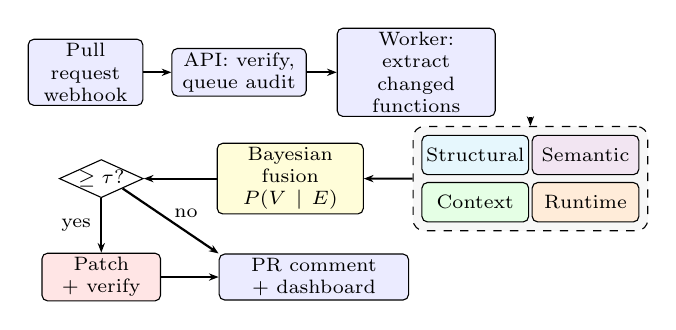
\begin{tikzpicture}[
  font=\scriptsize,
  box/.style={draw, rounded corners=2pt, align=center, minimum height=0.5cm,
              text width=#1, inner sep=1.5pt},
  box/.default=1.45cm,
  arr/.style={-{Stealth[length=3.5pt]}, thick}]
\node[box=1.35cm, fill=blue!8] (pr) at (0.4,0) {Pull request\\webhook};
\node[box=1.6cm, fill=blue!8] (api) at (2.35,0) {API: verify,\\queue audit};
\node[box=1.9cm, fill=blue!8] (ext) at (4.6,0) {Worker: extract\\changed functions};
\node[box=1.25cm, fill=cyan!10]   (s) at (5.35,-1.05) {Structural};
\node[box=1.25cm, fill=violet!10] (m) at (6.75,-1.05) {Semantic};
\node[box=1.25cm, fill=green!10]  (c) at (5.35,-1.65) {Context};
\node[box=1.25cm, fill=orange!15] (r) at (6.75,-1.65) {Runtime};
\begin{scope}[on background layer]
\node[draw, dashed, rounded corners, fill=gray!6, inner sep=3pt, fit=(s)(m)(c)(r)] (ag) {};
\end{scope}
\node[box=1.75cm, fill=yellow!15] (bay) at (3.0,-1.35) {Bayesian fusion\\$P(V\mid E)$};
\node[diamond, draw, aspect=2.2, inner sep=0pt, align=center] (dec) at (0.6,-1.35) {$\ge\tau$?};
\node[box=1.4cm, fill=red!10] (pat) at (0.6,-2.6) {Patch + verify};
\node[box=2.3cm, fill=blue!8] (out) at (3.3,-2.6) {PR comment\\+ dashboard};
\draw[arr] (pr) -- (api);
\draw[arr] (api) -- (ext);
\draw[arr] (ext.south -| ag.north) -- (ag.north);
\draw[arr] (ag.west) -- (bay.east);
\draw[arr] (bay) -- (dec);
\draw[arr] (dec) -- node[left]{yes} (pat);
\draw[arr] (pat) -- (out);
\draw[arr] (dec.south east) -- node[above right, inner sep=1pt]{no} (out.north west);
\end{tikzpicture}
\caption{Workflow of CodeSheriff. The four agents run blind.}
\label{fig:workflow}
\end{figure}

The CodeSheriff workflow (Fig.~\ref{fig:workflow}) consists of five
stages:
\begin{enumerate}
\item \textbf{Trigger:} opening or updating a pull request sends a webhook.
The API verifies its HMAC-SHA256 signature, records an audit, queues it and
replies within three seconds.
\item \textbf{Extraction:} a worker downloads the base and head files and
builds one unit per changed function using (\ref{eq:units}).
\item \textbf{Agent analysis:} the four agents analyse every unit
independently (Algorithm~\ref{alg:agents}).
\item \textbf{Fusion and decision:} the engine computes $P(V\mid E)$ and
the verdict (Algorithm~\ref{alg:fusion}); alerted findings go to the
patch stage (Algorithm~\ref{alg:patch}).
\item \textbf{Reporting:} one comment summarises the audit on the pull
request, and every statement, probability and per-agent factor is stored
for the dashboard.
\end{enumerate}

\subsection{Implementation}

CodeSheriff is a Python 3.12 monorepo. The API and the worker run as
separate processes with separate credentials: the API holds the webhook
secret, the worker holds the model key, and a queued task carries only an
audit identifier. Source code is kept in memory only; the database stores
findings and hashes. The main components are:
\begin{itemize}
\item \textbf{Backend:} FastAPI, Celery and Redis.
\item \textbf{Database:} PostgreSQL 16 with pgvector, SQLAlchemy, Alembic.
\item \textbf{Agents:} tree-sitter and networkx taint engine with Semgrep;
Gemini Flash-Lite ($n=3$); \texttt{bge-small-en-v1.5} embeddings;
Wasmtime with a WASI build of CPython.
\item \textbf{Dashboard:} Next.js, TypeScript and Recharts (read-only; the
threshold cannot be changed per repository).
\item \textbf{Quality:} 1249 tests, strict type checking, and import rules
that stop any agent from importing another agent or the database.
\end{itemize}

% =====================================================================
\section{Experimental Evaluation} \label{IMP}
% =====================================================================

\subsection{Experimental Setup}
The ground truth is a hand-written corpus of 76 Python functions in 38
\emph{twin pairs}: the same function once vulnerable and once fixed, over
ten CWEs (22, 78, 79, 89, 94, 502, 639, 798, 862, 918). Pairs are split by
pair into calibration (46 units), validation (14) and test (16). Ratios
are fitted only on calibration, the threshold is chosen only on
validation, and the test split is reserved for a single final run. No
agent can read a label. Because every case has a twin, the corpus is half
vulnerable, so the prior is \emph{declared} as $\pi=0.03$ and all metrics
are weighted so that vulnerable claims carry $3\%$ of the weight. The
experiments ran on an Intel Core i5 machine with 16~GB RAM using recorded
model responses, so every number is exactly reproducible.

Detection is measured by precision (P), recall (R) and $F_1$. Calibration
is measured by the Brier score~\cite{brier1950} and the expected
calibration error (ECE)~\cite{guo2017calibration}:
\begin{equation}
\mathrm{Brier}=\frac{1}{N}\sum_{i=1}^{N}(p_i-y_i)^2,\quad
\mathrm{ECE}=\sum_{b=1}^{10}\frac{|B_b|}{N}\bigl|\mathrm{freq}_b-\mathrm{conf}_b\bigr|
\label{eq:metrics}
\end{equation}
where $p_i$ is the predicted probability, $y_i\in\{0,1\}$ the true label,
and $B_b$ the claims in probability bin $b$. Lower is better for both.

\subsection{Individual Agents and Fitted Ratios}
Measured alone on the calibration split, the Structural agent detected
13/13 cases in its scope, the Context agent 5/5 and the Runtime agent 9/9,
each with zero false positives on the safe twins. The Semantic agent had
no hallucinated sinks, no successful prompt injection, and correctly
passed $94\%$ of safe twins. Table~\ref{tab:lr} gives the fitted ratios.
A medium structural detection makes a vulnerability $15.6\times$ more
likely, while structural silence makes it about $15\times$ less likely. A
low or medium semantic detection (one or two of three samples) has an LR
below $1$: such findings were more often safe. Voting would count them as
``yes''; the fitted ratio correctly treats them as weak evidence against.

\begin{table}[t]
\centering
\caption{Fitted likelihood ratios (-- : never observed, LR $=1$)}
\label{tab:lr}
\small
\setlength{\tabcolsep}{5pt}
\begin{tabular}{lcccc}
\toprule
Agent & High & Medium & Low & Silence \\
\midrule
Structural & 2.22 & 15.56 & --   & 0.065 \\
Semantic   & 9.48 & 0.56  & 0.74 & 0.304 \\
Context    & 2.00 & 4.00  & 2.00 & 0.167 \\
Runtime    & 6.92 & --    & --   & 0.115 \\
\bottomrule
\end{tabular}
\end{table}

\subsection{Comparative Analysis}
CodeSheriff is compared with two baselines built on the \emph{same} agent
statements, so only the combination rule differs: \emph{majority vote}
(share of agents that detected, abstentions ignored) and \emph{prior only}
(no agent). All use $\tau=0.227$. Table~\ref{tab:comparison} gives the
results.

\begin{table}[t]
\centering
\caption{Comparison using identical agent statements (best in bold)}
\label{tab:comparison}
\small
\setlength{\tabcolsep}{3.2pt}
\begin{tabular}{llccccc}
\toprule
Split & System & ECE$\downarrow$ & Brier$\downarrow$ & P$\uparrow$ & R$\uparrow$ & $F_1\uparrow$ \\
\midrule
Valid. & Prior only    & \textbf{0.000} & 0.029 & 0.000 & 0.000 & 0.000 \\
       & Majority vote & 0.141 & 0.059 & 0.076 & \textbf{1.000} & 0.142 \\
       & CodeSheriff   & 0.027 & \textbf{0.013} & \textbf{1.000} & 0.857 & \textbf{0.923} \\
\midrule
Calib. & Prior only    & \textbf{0.000} & 0.029 & 0.000 & 0.000 & 0.000 \\
       & Majority vote & 0.092 & 0.068 & 0.161 & \textbf{0.957} & 0.276 \\
       & CodeSheriff   & 0.009 & \textbf{0.010} & \textbf{1.000} & 0.696 & \textbf{0.821} \\
\bottomrule
\end{tabular}
\end{table}

\subsection{Ablation Analysis}
Each agent is removed in turn and treated as an abstention (factor $1$).
Fig.~\ref{fig:ablation} shows $F_1$ on both splits.

\begin{figure}[t]
\centering
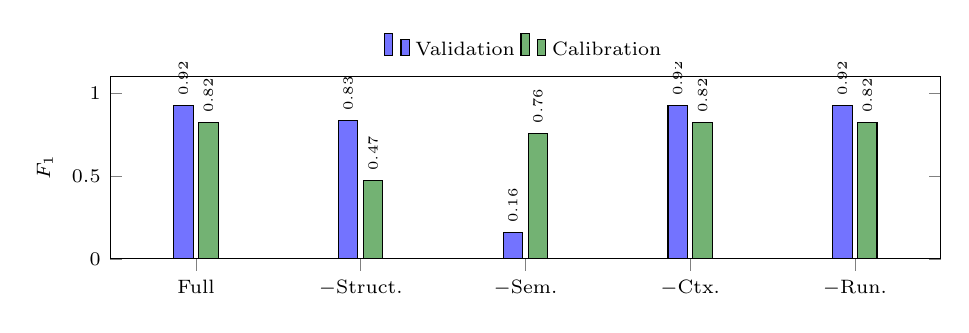
\begin{tikzpicture}
\begin{axis}[
  ybar, width=\columnwidth, height=3.9cm,
  bar width=7pt, enlarge x limits=0.13,
  ymin=0, ymax=1.1,
  symbolic x coords={Full,$-$Struct.,$-$Sem.,$-$Ctx.,$-$Run.},
  xtick=data, xtick pos=left, tick label style={font=\scriptsize},
  ylabel={$F_1$}, ylabel style={font=\scriptsize},
  nodes near coords, nodes near coords style={font=\tiny, rotate=90, anchor=west},
  every node near coord/.append style={/pgf/number format/fixed,/pgf/number format/precision=2},
  legend columns=2,
  legend style={font=\scriptsize, at={(0.5,1.03)}, anchor=south, draw=none}]
\addplot[fill=blue!55] coordinates {(Full,0.923) ($-$Struct.,0.833) ($-$Sem.,0.157) ($-$Ctx.,0.923) ($-$Run.,0.923)};
\addplot[fill=green!45!black!55] coordinates {(Full,0.821) ($-$Struct.,0.473) ($-$Sem.,0.757) ($-$Ctx.,0.821) ($-$Run.,0.821)};
\legend{Validation, Calibration}
\end{axis}
\end{tikzpicture}
\caption{Leave-one-agent-out ablation ($F_1$ at $\tau=0.227$).}
\label{fig:ablation}
\end{figure}

\subsection{Assumptions and Limitations}
The corpus is small, author-written, Python-only and limited to ten CWEs.
The validation split has only 15 claims and the threshold was chosen on
it, so its figures are selection-time estimates; the test split is not yet
evaluated. Semgrep has no Windows build, so the structural ratios describe
the taint engine alone. The $3\%$ base rate is declared, not measured.

% =====================================================================
\section{Results and Discussion} \label{RES}
% =====================================================================

On the validation split CodeSheriff reached $F_1=0.923$ with perfect
precision, alerting on 6 of 15 claims (Table~\ref{tab:comparison}).
Majority vote over the same statements found every vulnerability, but most
of its alerts were false ($F_1=0.142$) because it has no prior to hold one
agent's detection back, and it was five times worse calibrated (ECE $0.141$
against $0.027$). The prior-only baseline has a perfect ECE only because it
detects nothing; its Brier score ($0.029$ against $0.013$) exposes this.
The same ordering holds on the calibration split.

\begin{figure}[t]
\centering
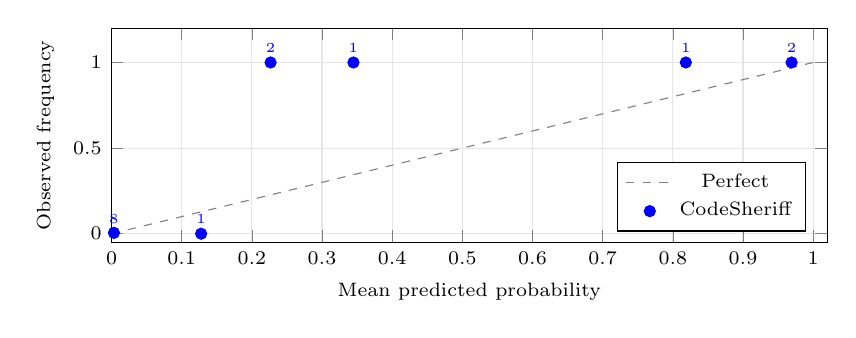
\begin{tikzpicture}
\begin{axis}[
  width=0.88\columnwidth, height=4.3cm,
  xmin=0, xmax=1.02, ymin=-0.05, ymax=1.2,
  xlabel={Mean predicted probability}, ylabel={Observed frequency},
  label style={font=\scriptsize}, tick label style={font=\scriptsize},
  legend style={font=\scriptsize, at={(0.97,0.05)}, anchor=south east},
  grid=major, grid style={gray!20}]
\addplot[dashed, gray, domain=0:1] {x};
\addplot[only marks, mark=*, blue, mark size=2pt,
  nodes near coords, point meta=explicit symbolic,
  every node near coord/.append style={font=\tiny, anchor=south}]
  coordinates {
  (0.0034,0.0050) [8]
  (0.1277,0.0)    [1]
  (0.2267,1.0)    [2]
  (0.3448,1.0)    [1]
  (0.8185,1.0)    [1]
  (0.9693,1.0)    [2]};
\legend{Perfect, CodeSheriff}
\end{axis}
\end{tikzpicture}
\caption{Reliability diagram, validation split (labels: claims per bin).}
\label{fig:reliability}
\end{figure}

Fig.~\ref{fig:reliability} is the reliability diagram. Most claims receive
a very low probability and are indeed safe, and all high-probability claims
are vulnerable. The two middle bins lie above the diagonal, meaning the
system was slightly \emph{under}-confident there, but they hold only one or
two claims each and carry little weight.

The ablation (Fig.~\ref{fig:ablation}) shows that the two splits disagree
about which agent matters most. On validation, removing the Semantic agent
drops $F_1$ from $0.923$ to $0.157$; on calibration, removing the
Structural agent drops it from $0.821$ to $0.473$. No single agent is
enough on both splits, which supports using heterogeneous agents. Removing
the Context or Runtime agent leaves every decision unchanged; this is a
null result, not redundancy, since both have narrow scopes and mostly
confirm decisions another agent already made.

% =====================================================================
\section{Conclusion} \label{CON}
% =====================================================================

This paper presented CodeSheriff, a pull-request security auditor in which
four agents built on different techniques analyse each changed function
independently, and a Bayesian engine turns their statements into a
calibrated probability. The design separates ``found nothing'' from
``could not look'', and fits every ratio and the threshold on labelled
data. On the validation split it reached $F_1=0.923$ with perfect
precision and ECE $0.027$, while majority voting over identical
statements reached only $0.142$. Unlike related
systems~\cite{ref2,ref1,ref16,ref6}, it pairs verified patch suggestions
with a probability whose reliability is itself measured.

\section{Future Scope}
The test split will be evaluated once on a Linux image where Semgrep is
active, and Semgrep, Bandit and a single-pass LLM will be scored under the
same protocol. The corpus will be enlarged with real vulnerability-fixing
commits, and support extended to JavaScript and TypeScript.

\section*{Acknowledgment}
The authors thank the Department of Information Technology, G H Raisoni
College of Engineering and Management, Pune, for its resources, and the
project guides for their support.

\balance
\bibliographystyle{IEEEtran}
\bibliography{references}

\end{document}
